\documentclass[]{article}
\usepackage{lmodern}
\usepackage{amssymb,amsmath}
\usepackage{ifxetex,ifluatex}
\usepackage{fixltx2e} % provides \textsubscript
\ifnum 0\ifxetex 1\fi\ifluatex 1\fi=0 % if pdftex
  \usepackage[T1]{fontenc}
  \usepackage[utf8]{inputenc}
\else % if luatex or xelatex
  \ifxetex
    \usepackage{mathspec}
  \else
    \usepackage{fontspec}
  \fi
  \defaultfontfeatures{Ligatures=TeX,Scale=MatchLowercase}
\fi
% use upquote if available, for straight quotes in verbatim environments
\IfFileExists{upquote.sty}{\usepackage{upquote}}{}
% use microtype if available
\IfFileExists{microtype.sty}{%
\usepackage{microtype}
\UseMicrotypeSet[protrusion]{basicmath} % disable protrusion for tt fonts
}{}
\usepackage[margin=1in]{geometry}
\usepackage{hyperref}
\hypersetup{unicode=true,
            pdftitle={Practical 2 - Testing and Debugging},
            pdfauthor={MT4113},
            pdfborder={0 0 0},
            breaklinks=true}
\urlstyle{same}  % don't use monospace font for urls
\usepackage{color}
\usepackage{fancyvrb}
\newcommand{\VerbBar}{|}
\newcommand{\VERB}{\Verb[commandchars=\\\{\}]}
\DefineVerbatimEnvironment{Highlighting}{Verbatim}{commandchars=\\\{\}}
% Add ',fontsize=\small' for more characters per line
\usepackage{framed}
\definecolor{shadecolor}{RGB}{248,248,248}
\newenvironment{Shaded}{\begin{snugshade}}{\end{snugshade}}
\newcommand{\KeywordTok}[1]{\textcolor[rgb]{0.13,0.29,0.53}{\textbf{#1}}}
\newcommand{\DataTypeTok}[1]{\textcolor[rgb]{0.13,0.29,0.53}{#1}}
\newcommand{\DecValTok}[1]{\textcolor[rgb]{0.00,0.00,0.81}{#1}}
\newcommand{\BaseNTok}[1]{\textcolor[rgb]{0.00,0.00,0.81}{#1}}
\newcommand{\FloatTok}[1]{\textcolor[rgb]{0.00,0.00,0.81}{#1}}
\newcommand{\ConstantTok}[1]{\textcolor[rgb]{0.00,0.00,0.00}{#1}}
\newcommand{\CharTok}[1]{\textcolor[rgb]{0.31,0.60,0.02}{#1}}
\newcommand{\SpecialCharTok}[1]{\textcolor[rgb]{0.00,0.00,0.00}{#1}}
\newcommand{\StringTok}[1]{\textcolor[rgb]{0.31,0.60,0.02}{#1}}
\newcommand{\VerbatimStringTok}[1]{\textcolor[rgb]{0.31,0.60,0.02}{#1}}
\newcommand{\SpecialStringTok}[1]{\textcolor[rgb]{0.31,0.60,0.02}{#1}}
\newcommand{\ImportTok}[1]{#1}
\newcommand{\CommentTok}[1]{\textcolor[rgb]{0.56,0.35,0.01}{\textit{#1}}}
\newcommand{\DocumentationTok}[1]{\textcolor[rgb]{0.56,0.35,0.01}{\textbf{\textit{#1}}}}
\newcommand{\AnnotationTok}[1]{\textcolor[rgb]{0.56,0.35,0.01}{\textbf{\textit{#1}}}}
\newcommand{\CommentVarTok}[1]{\textcolor[rgb]{0.56,0.35,0.01}{\textbf{\textit{#1}}}}
\newcommand{\OtherTok}[1]{\textcolor[rgb]{0.56,0.35,0.01}{#1}}
\newcommand{\FunctionTok}[1]{\textcolor[rgb]{0.00,0.00,0.00}{#1}}
\newcommand{\VariableTok}[1]{\textcolor[rgb]{0.00,0.00,0.00}{#1}}
\newcommand{\ControlFlowTok}[1]{\textcolor[rgb]{0.13,0.29,0.53}{\textbf{#1}}}
\newcommand{\OperatorTok}[1]{\textcolor[rgb]{0.81,0.36,0.00}{\textbf{#1}}}
\newcommand{\BuiltInTok}[1]{#1}
\newcommand{\ExtensionTok}[1]{#1}
\newcommand{\PreprocessorTok}[1]{\textcolor[rgb]{0.56,0.35,0.01}{\textit{#1}}}
\newcommand{\AttributeTok}[1]{\textcolor[rgb]{0.77,0.63,0.00}{#1}}
\newcommand{\RegionMarkerTok}[1]{#1}
\newcommand{\InformationTok}[1]{\textcolor[rgb]{0.56,0.35,0.01}{\textbf{\textit{#1}}}}
\newcommand{\WarningTok}[1]{\textcolor[rgb]{0.56,0.35,0.01}{\textbf{\textit{#1}}}}
\newcommand{\AlertTok}[1]{\textcolor[rgb]{0.94,0.16,0.16}{#1}}
\newcommand{\ErrorTok}[1]{\textcolor[rgb]{0.64,0.00,0.00}{\textbf{#1}}}
\newcommand{\NormalTok}[1]{#1}
\usepackage{graphicx,grffile}
\makeatletter
\def\maxwidth{\ifdim\Gin@nat@width>\linewidth\linewidth\else\Gin@nat@width\fi}
\def\maxheight{\ifdim\Gin@nat@height>\textheight\textheight\else\Gin@nat@height\fi}
\makeatother
% Scale images if necessary, so that they will not overflow the page
% margins by default, and it is still possible to overwrite the defaults
% using explicit options in \includegraphics[width, height, ...]{}
\setkeys{Gin}{width=\maxwidth,height=\maxheight,keepaspectratio}
\IfFileExists{parskip.sty}{%
\usepackage{parskip}
}{% else
\setlength{\parindent}{0pt}
\setlength{\parskip}{6pt plus 2pt minus 1pt}
}
\setlength{\emergencystretch}{3em}  % prevent overfull lines
\providecommand{\tightlist}{%
  \setlength{\itemsep}{0pt}\setlength{\parskip}{0pt}}
\setcounter{secnumdepth}{0}
% Redefines (sub)paragraphs to behave more like sections
\ifx\paragraph\undefined\else
\let\oldparagraph\paragraph
\renewcommand{\paragraph}[1]{\oldparagraph{#1}\mbox{}}
\fi
\ifx\subparagraph\undefined\else
\let\oldsubparagraph\subparagraph
\renewcommand{\subparagraph}[1]{\oldsubparagraph{#1}\mbox{}}
\fi

%%% Use protect on footnotes to avoid problems with footnotes in titles
\let\rmarkdownfootnote\footnote%
\def\footnote{\protect\rmarkdownfootnote}

%%% Change title format to be more compact
\usepackage{titling}

% Create subtitle command for use in maketitle
\newcommand{\subtitle}[1]{
  \posttitle{
    \begin{center}\large#1\end{center}
    }
}

\setlength{\droptitle}{-2em}

  \title{Practical 2 - Testing and Debugging}
    \pretitle{\vspace{\droptitle}\centering\huge}
  \posttitle{\par}
    \author{MT4113}
    \preauthor{\centering\large\emph}
  \postauthor{\par}
      \predate{\centering\large\emph}
  \postdate{\par}
    \date{28 September 2018}


\begin{document}
\maketitle

\section{How do you know your code
works?}\label{how-do-you-know-your-code-works}

\begin{itemize}
\tightlist
\item
  Writing code is only the first step
\item
  As a programmer, you need to determine if your code performs as you
  intended
\end{itemize}

\subsection{Types of code errors}\label{types-of-code-errors}

\begin{itemize}
\tightlist
\item
  syntax errors

  \begin{itemize}
  \tightlist
  \item
    code not consistent with the programming language
  \item
    not always obvious in \texttt{R}
  \end{itemize}
\end{itemize}

\begin{Shaded}
\begin{Highlighting}[]
\NormalTok{bad <-}\StringTok{ }\ControlFlowTok{function}\NormalTok{(}\DataTypeTok{x =} \DecValTok{7}\NormalTok{) \{}
  \ControlFlowTok{if}\NormalTok{ (x }\OperatorTok{>}\StringTok{ }\DecValTok{10}\NormalTok{) \{}
\NormalTok{    y <-}\StringTok{ }\KeywordTok{ln}\NormalTok{(}\DecValTok{22}\NormalTok{)}
\NormalTok{  \} }\ControlFlowTok{else}\NormalTok{ \{}
\NormalTok{    y <-}\StringTok{ }\DecValTok{7}
\NormalTok{  \}}
  \KeywordTok{return}\NormalTok{(y)}
\NormalTok{\}}

\NormalTok{this.x <-}\StringTok{ }\DecValTok{4}
\NormalTok{answer <-}\StringTok{ }\KeywordTok{bad}\NormalTok{(this.x)}
\KeywordTok{print}\NormalTok{(answer)}
\end{Highlighting}
\end{Shaded}

\begin{verbatim}
## [1] 7
\end{verbatim}

\begin{itemize}
\tightlist
\item
  logic errors

  \begin{itemize}
  \tightlist
  \item
    topic of today's practical
  \end{itemize}
\item
  numerical errors (overflows/underflows/floating point problems)

  \begin{itemize}
  \tightlist
  \item
    limitation of manner numbers are stored in computers
  \item
    topic of next Wednesday's lecture
  \end{itemize}
\end{itemize}

\section{Code testing}\label{code-testing}

\subsection{How to build tests}\label{how-to-build-tests}

\begin{itemize}
\tightlist
\item
  do you know what your code should produce?

  \begin{itemize}
  \tightlist
  \item
    result from a textbook or paper
  \item
    result in a more simple case
  \item
    result from previous version of your code
  \end{itemize}
\item
  how does code behave with special cases?

  \begin{itemize}
  \tightlist
  \item
    input is 0
  \item
    input is NA
  \item
    input is gigantic, gigantically negative
  \end{itemize}
\item
  build the tests prior to building the code (?!)

  \begin{itemize}
  \tightlist
  \item
    code is created so as to pass the tests
  \end{itemize}
\end{itemize}

\section{Code does not work, where is the
error?}\label{code-does-not-work-where-is-the-error}

\begin{itemize}
\tightlist
\item
  Using modular programming, you have created code as a series of
  functions
\item
  Process of finding error summarised as:
\end{itemize}

\begin{quote}
``\ldots{} confirming, one by one, many things you \emph{believe} to be
true about your code, actually \emph{are} true. When you find a belief
that is \emph{not} true, you have found a clue to the location of a
bug.'' -- Norman Matloff
\end{quote}

\begin{itemize}
\tightlist
\item
  examine results of each function, when result does not conform to
  expectation, performance of that function is in doubt.
\end{itemize}

\subsection{A function to debug}\label{a-function-to-debug}

Here is a small bit of code, from
\href{http://library.st-andrews.ac.uk/search~S5?/amatloff\&keyword-selector=author/amatloff/1\%2C4\%2C7\%2CB/frameset\&FF=amatloff+norman+s+author\&1\%2C1\%2C}{Matloff
(2011, Chapter 13)}. The purpose of the function \texttt{findruns} is to
examine vectors containing binary values (0,1), and locate runs of
consecutive \texttt{1s} of given length.

The algorithm:

\begin{itemize}
\tightlist
\item
  Start at beginning of the vector
\item
  move sequentially in blocks of length \emph{k}
\item
  test whether all elements within the block are 1's

  \begin{itemize}
  \tightlist
  \item
    if yes, denote first element of block as beginning point of a `run'
  \item
    if no, slide window along to next block
  \end{itemize}
\item
  terminate when last element of block corresponds to last element in
  vector
\end{itemize}

Example run:

\begin{Shaded}
\begin{Highlighting}[]
\NormalTok{test.case <-}\StringTok{ }\KeywordTok{c}\NormalTok{(}\DecValTok{1}\NormalTok{, }\DecValTok{0}\NormalTok{, }\DecValTok{0}\NormalTok{, }\DecValTok{1}\NormalTok{, }\DecValTok{1}\NormalTok{, }\DecValTok{1}\NormalTok{, }\DecValTok{0}\NormalTok{, }\DecValTok{1}\NormalTok{, }\DecValTok{1}\NormalTok{)}
\KeywordTok{findruns.correct}\NormalTok{(test.case, }\DecValTok{2}\NormalTok{)}
\end{Highlighting}
\end{Shaded}

\begin{verbatim}
## [1] 4 5 8
\end{verbatim}

indicating runs of length 2 begin in positions 4, 5, and 8.

Imagine however, you have been presented with code shown here:

\begin{Shaded}
\begin{Highlighting}[]
\NormalTok{findruns <-}\StringTok{ }\ControlFlowTok{function}\NormalTok{(x, k) \{}
\NormalTok{  n <-}\StringTok{ }\KeywordTok{length}\NormalTok{(x)}
\NormalTok{  runs <-}\StringTok{ }\OtherTok{NULL}
  \ControlFlowTok{for}\NormalTok{ (i }\ControlFlowTok{in} \DecValTok{1}\OperatorTok{:}\NormalTok{(n }\OperatorTok{-}\StringTok{ }\NormalTok{k)) \{}
    \ControlFlowTok{if}\NormalTok{ (}\KeywordTok{all}\NormalTok{(x[i}\OperatorTok{:}\NormalTok{i }\OperatorTok{+}\StringTok{ }\NormalTok{k }\OperatorTok{-}\StringTok{ }\DecValTok{1}\NormalTok{] }\OperatorTok{==}\StringTok{ }\DecValTok{1}\NormalTok{)) runs <-}\StringTok{ }\KeywordTok{c}\NormalTok{(runs, i)}
\NormalTok{  \}}
  \KeywordTok{return}\NormalTok{(runs)}
\NormalTok{\}}
\end{Highlighting}
\end{Shaded}

when this code is presented with the test case from above:

\begin{Shaded}
\begin{Highlighting}[]
\KeywordTok{findruns}\NormalTok{(test.case, }\DecValTok{2}\NormalTok{)}
\end{Highlighting}
\end{Shaded}

\begin{verbatim}
## [1] 3 4 5 7
\end{verbatim}

Erroneous results are discovered. Two of the locations are detected
correctly, but another run is erroneously reported, and the final run is
mis-located.

\section{Your task}\label{your-task}

Diagnose and correct the problems within these eight lines of code.

\subsection{Classic debugging
strategies}\label{classic-debugging-strategies}

\begin{itemize}
\item
  Trial and error: maybe you can guess what is wrong based on the output
\item
  Make your function global: set global values for the arguments and
  step through the function
\item
  Add \texttt{print()} statements: use to print object values as the
  function progresses
\item
  More information about debugging in general:
  \href{http://adv-r.had.co.nz/Exceptions-Debugging.html}{Advanced R:
  Exceptions and Debugging}
\end{itemize}

\subsection{RStudio debugger}\label{rstudio-debugger}

An extensive \emph{how to} description of using the R Studio interactive
debugger is at the
\href{https://support.rstudio.com/hc/en-us/articles/205612627-Debugging-with-RStudio}{R
Studio support website}.

R Studio have also produced \href{https://vimeo.com/99375765}{a
10-minute video describing the use of their debugger.} Please use
headphones if you choose to watch this in class!

Using the debugger consists of pausing execution of your code. This is
done in one of several ways

\begin{itemize}
\tightlist
\item
  breakpoints - places in your code where you wish execution to pause.
  These can be set using

  \begin{itemize}
  \tightlist
  \item
    editor window and mouse (click to left of line number)
    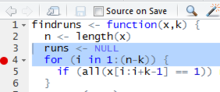
\includegraphics{screen1.png}
  \item
    insert \texttt{browser()} call in code
  \end{itemize}
\item
  if suspicious line of code is not known, use menu command:
  \texttt{Debug\ \textbar{}\ On\ Error\ \textbar{}\ Break\ in\ Code}
\end{itemize}

\subsection{The environment pane}\label{the-environment-pane}

When the debugger is invoked, the environment pane shows the state of
the current environment. Above the Values in the environment pane, is a
pull-down menu showing the sequence of environments that will be
searched to find object values.

\begin{figure}
\centering
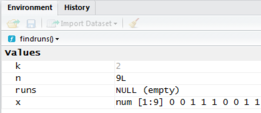
\includegraphics{enviro.png}
\caption{The local environment in function findruns.}
\end{figure}

We discussed this \texttt{search\ chain} in Lecture 3 in the context of
searching through loaded packages to find a function.

Not only are objects in the current environment that have been assigned
a value displayed, but also values of arguments that have been passed
into the function \emph{but not yet evaluated} (called ``promises'') are
also show in grey (the argument \texttt{k} in this case).

\begin{figure}
\centering
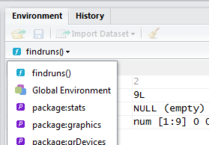
\includegraphics{envir-stack.png}
\caption{The search path, or environment stack inside findruns.}
\end{figure}

\subsection{Code and console panes}\label{code-and-console-panes}

When debugging, the code pane highlights the location as code is
executed. That way flow of control is apparent to you as you step
thorough your code.

How to step through your code you might ask. Note the console pane has
been changed when the debugger is operating.

\begin{figure}
\centering
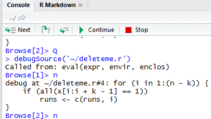
\includegraphics{browse-console.png}
\caption{Console pane when debugger is active.}
\end{figure}

Stepping through lines of code is done using either \texttt{next} for a
single line, \texttt{run\ to\ end} of function or loop or
\texttt{continue} until next breakpoint is encountered. As the code is
processed, you can see resulting changes to the values in the
environment. You can also change the values of objects in the
environment by typing assignment operators after the
\texttt{Browse{[}2{]}\textgreater{}} prompt.

By the way the \texttt{{[}2{]}} indicates the depth to which the code
you are executing is nested within R's environment. \texttt{{[}1{]}}
indicates code is in the \texttt{Global\ Environment}, \texttt{{[}2{]}}
is inside a function called from the Global Environment,
\texttt{{[}3{]}} would be inside a function called from a function
called from the Global Environment.

With your new friend, the debugger, set about your task of

\begin{itemize}
\tightlist
\item
  finding the error(s) within the function \texttt{findruns()}
\item
  correct those errors so the function performs as expected
\end{itemize}

\begin{center}\rule{0.5\linewidth}{\linethickness}\end{center}

\begin{center}\rule{0.5\linewidth}{\linethickness}\end{center}

\section{Extra practice in constructing random deviates (if you
wish)}\label{extra-practice-in-constructing-random-deviates-if-you-wish}

Remember the family of \texttt{d}, \texttt{p}, \texttt{q}, \texttt{r}
functions for statistical distributions? They produce the probability
density function, cumulative distribution function, inverse cumulative
distribution function and random deviates respectively. These functions
are provided in R for a number of statistical distributions: normal,
Students t, \(\chi^2\), F, \ldots{} But one (of many) distributions that
do not have these functions is the Pareto (named after an Italian
scientist). It is a two-parameter distribution that has found uses in
modelling the upper tail of wealth distribution.

Create PDF \(f(x)\), CDF \(F(x)\) and inverse CDF \(F^{-1}(p)\)
functions based upon this equations:

\[
f(x;\alpha, x_0) =  \left\{
                \begin{aligned}
                  \frac{\alpha-1}{x_0}\left( \frac{x}{x_0} \right)^{-\alpha}, & x \ge x_0\\
                  0, & x \lt x_0
                \end{aligned}
              \right.
\] \[
F(x; \alpha, x_0) = 1 - \left( \frac{x}{x_0}\right)^{-\alpha + 1}
\]

\[
F^{-1}(p; \alpha, x_0) = x_0 \left (1-p \right )^{-\frac{1}{\alpha-1}}
\]

Having written those functions, the remaining function would be
\texttt{rpareto()} to generate deviates distributed as Pareto. However,
there is no formula to produce these deviates. Consequently, we resort
to using a method of producing random deviates called \emph{quantile
transform} method or \emph{inverse transform sampling}.

Here is a one-sentence description of the \emph{quantile transform}.
Given the y-range of \(F(x; \alpha, x_0)\) is {[}0,1{]}, by generating
random deviates \(\sim U(0,1)\) and passing them as arguments to
\(F^{-1}(p; \alpha, x_0)\). With that hint, complete the fourth function
\texttt{rpareto()} for this distribution.

For example, this figure depicts producing a value from \(\sim U(0,1)\)
(0.6 in this case) and projecting that value from the y-axis, through
the CDF, onto the x-axis to produce a random deviate from the Pareto
distribution with parameters \(\alpha=1.3\) and \(x_0=1\), resulting in
a Pareto-distributed deviate value of 32.

\includegraphics{prac02-debugging-2018_files/figure-latex/invcdf-1.pdf}

\subsection{Extra extra practice}\label{extra-extra-practice}

What checks should be placed upon the arguments coming into each of
these functions?


\end{document}
